%% Преамбула TeX-файла

% 1. Стиль и язык
\documentclass[utf8x, 14pt]{G7-32} % Стиль (по умолчанию будет 14pt)

% Остальные стандартные настройки убраны в preamble.inc.tex.
\sloppy

% Настройки стиля ГОСТ 7-32
% Для начала определяем, хотим мы или нет, чтобы рисунки и таблицы нумеровались в пределах раздела, или нам нужна сквозная нумерация.
\EqInChapter % формулы будут нумероваться в пределах раздела
\TableInChapter % таблицы будут нумероваться в пределах раздела
\PicInChapter % рисунки будут нумероваться в пределах раздела

% Добавляем гипертекстовое оглавление в PDF
\usepackage[
bookmarks=true, colorlinks=true, unicode=true,
urlcolor=black,linkcolor=black, anchorcolor=black,
citecolor=black, menucolor=black, filecolor=black,
]{hyperref}

\AfterHyperrefFix

% Альтернативный Пакет для создания списка терминов со ссылками на них
\usepackage{glossaries}
\usepackage[stylemods,style=long3col]{glossaries-extra}
\setabbreviationstyle[acronym]{long-short}
\makenoidxglossaries


\usepackage{microtype}% полезный пакет для микротипографии, увы под xelatex мало чего умеет, но под pdflatex хорошо улучшает читаемость

% Тире могут быть невидимы в Adobe Reader
\ifInvisibleDashes
\MakeDashesBold
\fi

\usepackage{graphicx}   % Пакет для включения рисунков

% С такими оно полями оно работает по-умолчанию:
% \RequirePackage[left=20mm,right=10mm,top=20mm,bottom=20mm,headsep=0pt,includefoot]{geometry}
% Если вас тошнит от поля в 10мм --- увеличивайте до 20-ти, ну и про переплёт не забывайте:
\geometry{right=20mm}
\geometry{left=30mm}
\geometry{bottom=20mm}
\geometry{ignorefoot}% считать от нижней границы текста


% Пакет Tikz
\usepackage{tikz}
\usetikzlibrary{arrows,positioning,shadows}

% Произвольная нумерация списков.
\usepackage{enumerate}

% ячейки в несколько строчек
\usepackage{multirow}

% itemize внутри tabular
\usepackage{paralist,array}

%\setlength{\parskip}{1ex plus0.5ex minus0.5ex} % разрыв между абзацами
\setlength{\parskip}{1ex} % разрыв между абзацами
\usepackage{blindtext}

% Центрирование подписей к плавающим окружениям
%\usepackage[justification=centering]{caption}

\usepackage{newfloat}
\DeclareFloatingEnvironment[
placement={!ht},
name=Equation
]{eqndescNoIndent}
\edef\fixEqndesc{\noexpand\setlength{\noexpand\parindent}{\the\parindent}\noexpand\setlength{\noexpand\parskip}{\the\parskip}}
\newenvironment{eqndesc}[1][!ht]{%
    \begin{eqndescNoIndent}[#1]%
\fixEqndesc%
}
{\end{eqndescNoIndent}}




% Подключение словарей терминов и сокращений
% \newglossaryentry{api}{name={API},description={application programming interface ""--- внешний интерфейс взаимодействия с приложением \cite{law_RU_GradoCodex}}}

\newacronym{api}{API}{application programming interface ""--- внешний интерфейс взаимодействия с приложением \cite{law_RU_GradoCodex}}
\newacronym{factor.usefulEnergy}{КПД}{коэффициент полезного действия}

\newacronym{law.lna}{НПА}{нормативно-правовой акт}


\newglossaryentry{coolt}{name={Coolterm},description={звучит как название фирмы}}

% \usepackage{./assets/shema_bycountry_energyefficiency_compare}

\begin{document}
% Настройки листингов.
\ifPDFTeX
% % 8 Листинги

\usepackage{listings}

% Значения по умолчанию
\lstset{
  basicstyle= \footnotesize,
  breakatwhitespace=true,% разрыв строк только на whitespacce
  breaklines=true,       % переносить длинные строки
%   captionpos=b,          % подписи снизу -- вроде не надо
  inputencoding=koi8-r,
  numbers=left,          % нумерация слева
  numberstyle=\footnotesize,
  showspaces=false,      % показывать пробелы подчеркиваниями -- идиотизм 70-х годов
  showstringspaces=false,
  showtabs=false,        % и табы тоже
  stepnumber=1,
  tabsize=4,              % кому нужны табы по 8 символов?
  frame=single
}

% Стиль для псевдокода: строчки обычно короткие, поэтому размер шрифта побольше
\lstdefinestyle{pseudocode}{
  basicstyle=\small,
  keywordstyle=\color{black}\bfseries\underbar,
  language=Pseudocode,
  numberstyle=\footnotesize,
  commentstyle=\footnotesize\it
}

% Стиль для обычного кода: маленький шрифт
\lstdefinestyle{realcode}{
  basicstyle=\scriptsize,
  numberstyle=\footnotesize
}

% Стиль для коротких кусков обычного кода: средний шрифт
\lstdefinestyle{simplecode}{
  basicstyle=\footnotesize,
  numberstyle=\footnotesize
}

% Стиль для BNF
\lstdefinestyle{grammar}{
  basicstyle=\footnotesize,
  numberstyle=\footnotesize,
  stringstyle=\bfseries\ttfamily,
  language=BNF
}

% Определим свой язык для написания псевдокодов на основе Python
\lstdefinelanguage[]{Pseudocode}[]{Python}{
  morekeywords={each,empty,wait,do},% ключевые слова добавлять сюда
  morecomment=[s]{\{}{\}},% комменты {а-ля Pascal} смотрятся нагляднее
  literate=% а сюда добавлять операторы, которые хотите отображать как мат. символы
    {->}{\ensuremath{$\rightarrow$}~}2%
    {<-}{\ensuremath{$\leftarrow$}~}2%
    {:=}{\ensuremath{$\leftarrow$}~}2%
    {<--}{\ensuremath{$\Longleftarrow$}~}2%
}[keywords,comments]

% Свой язык для задания грамматик в BNF
\lstdefinelanguage[]{BNF}[]{}{
  morekeywords={},
  morecomment=[s]{@}{@},
  morestring=[b]",%
  literate=%
    {->}{\ensuremath{$\rightarrow$}~}2%
    {*}{\ensuremath{$^*$}~}2%
    {+}{\ensuremath{$^+$}~}2%
    {|}{\ensuremath{$|$}~}2%
}[keywords,comments,strings]

% Подписи к листингам на русском языке.
\renewcommand\lstlistingname{Листинг}
\renewcommand\lstlistlistingname{Листинги}

\else
\usepackage{local-minted}
\usepackage{lastpage}
\fi


% Полезные макросы листингов.
% Любимые команды
\newcommand{\Code}[1]{\textbf{#1}}


% Стиль титульного листа и заголовки

%\NirEkz{Экз. 3}                                  % Раскоментировать если не требуется
%\NirGrif{Секретно}                % Наименование грифа

%\gosttitle{Gost7-32}       % Шаблон титульной страницы, по умолчанию будет ГОСТ 7.32-2001, 
% Варианты GostRV15-110 или Gost7-32 
 
\NirOrgLongName{МИНОБРНАУКИ РОССИИ \\
% Российской Федерации\par
Федеральное государственное автономное образовательное учреждение высшего
образования
«Северо-Восточный федеральный университет имени М.К.Аммосова»
(СВФУ) \\
Инженерно-технический институт
}                                           %% Полное название организации

\NirUdk{УДК № 69}
% \NirGosNo{№ госрегистрации 01970006723}
%\NirInventarNo{Инв. № ??????}

%\NirConfirm{Согласовано}                  % Смена УТВЕРЖДАЮ
\NirBoss[.49]{Проректор по науке
и инновациям СВФУ}{Е.Э. Соловьев}            %% Заказчик, утверждающий НИР


%\NirReportName{Научно-технический отчет}   % Можно поменять тип отчета
%\NirAbout{О составной части \par опытно-конструкторской работы} %Можно изменить о чем отчет

%\NirPartNum{Часть}{1}                      % Часть номер

%\NirBareSubject{}                  % Убирает по теме если раскоментить

% \NirIsAnnotacion{АННОТАЦИОННЫЙ }         %% Раскомментируйте, если это аннотационный отчёт
%\NirStage{промежуточный}{Этап \No 1}{} %%% Этап НИР: {номер этапа}{вид отчёта - промежуточный или заключительный}{название этапа}
%\NirStage{}{}{} %%% Этап НИР: {номер этапа}{вид отчёта - промежуточный или 

\Nir{Разработка научно-обоснованных решений в проектировании, строительстве и
эксплуатации арктических поселений, отвечающих современным стандартам устойчивого
развития и комфортности проживания. Этап 1}

\NirSubject{Обзор и оценка решений по строительству и градостроительных принципов в условиях Арктики}                                   % Наименование темы
%\NirFinal{}                        % Заключительный, если закоментировать то промежуточный
%\finalname{итоговый}               % Название финального отчета (Заключительный) 
%\NirCode{Шифр\,---\,САПР-РЛС-ФИЗТЕХ-1} % Можно задать шифр как в ГОСТ 15.110
\NirCode{Шифр темы: ГК № 8019}

\NirManager{Руководитель темы, \\ Директор ИТИ, д.т.н., доцент}{Т.А. Корнилов  } %% Название руководителя
\NirIsp{Ответственный исполнитель, Менеджер УМО ИТИ, к.т.н.}{А.Л. Попов} %% Название руководителя

\NirYear{2022}%% если нужно поменять год отчёта; если закомментировано, ставится текущий год
\NirTown{Якутск, }                           %% город, в котором написан отчёт




\frontmatter % выключает нумерацию ВСЕГО; здесь начинаются ненумерованные главы: реферат, введение, глоссарий, сокращения и прочее.

\maketitle %создает титульную страницу


\begin{executors}
\personalSignature{Первый исполнитель}{ФИО}

\personalSignature{Второй исполнитель}{ФИО}
\end{executors}

% \listoffigures                         % Список рисунков

%\listoftables                          % Список таблиц

%\NormRefs % Нормативные ссылки 
% Команды \breakingbeforechapters и \nonbreakingbeforechapters
% управляют разрывом страницы перед главами.
% По-умолчанию страница разрывается.

% \nobreakingbeforechapters
% \breakingbeforechapters

% % Также можно использовать \Referat, как в оригинале


\begin{abstract}

    Отчет содержит \pageref{LastPage}\,стр.%
    \ifnum \totfig >0
    , \totfig~рис.%
    \fi
    \ifnum \tottab >0
    , \tottab~табл.%
    \fi
    %
    \ifnum \totbib >0
    , \totbib~источн.%
    \fi
    %
    \ifnum \totapp >0
    , \totapp~прил.%
    \else
    .%
    \fi


    Это пример каркаса расчётно-пояснительной записки, желательный к использованию в РПЗ проекта по курсу РСОИ
    \nocite{*}.

    Данный опус, как и более новые версии этого документа, можно взять по адресу (\url{https://github.com/latex-g7-32/latex-g7-32}).

    Текст в документе носит совершенно абстрактный характер.

\end{abstract}

%%% Local Variables: 
%%% mode: latex
%%% TeX-master: "rpz"
%%% End: 


\tableofcontents

% \Abbreviations
% \printnomenclature % Автоматический список сокращений

% Распечатка списка сокращений
% \setacronymstyle{long-short}
% \printnoidxglossaries
\printnoidxglossary[sort=word]% main glossary
% \printnoidxglossary[type=symbols,% symbols glossary
% sort=use]

% \Defines % Словарь терминов
\begin{description}
\item[Распределённый] Слово, которое нельзя употреблять. Но надо протестировать длинные строки в глоссарии.
\end{description}

%%% Local Variables:
%%% mode: latex
%%% TeX-master: "rpz"
%%% End:

% \Abbreviations %% Список обозначений и сокращений в тексте
\begin{description}
\item[АИС] Автоматизированная информационная система. Но надо протестировать длинные строки в определениях.
\end{description}

%%% Local Variables:
%%% mode: latex
%%% TeX-master: "rpz"
%%% End:


% \Introduction

Целью работы является создание всякой всячины. Для достижения поставленной цели необходимо решить следующие задачи:

\begin{itemize}
\item проанализировать существующую всячину;
\item спроектировать свою, новую всячину;
\item изготовить всякую всячину;
\item проверить её работоспособность.
\end{itemize}

Проверяем как у нас работают сокращения, обозначения и определения "---
MAX, 
\Abbrev{MAX}{Maximum ""--- максимальное значение параметра}
API 
\Abbrev{API}{application programming interface ""--- внешний интерфейс взаимодействия с приложением}
с обратным прокси.
\Define{Обратный прокси}{тип прокси-сервера, который ретранслирует}





\mainmatter % это включает нумерацию глав и секций в документе ниже

% \chapter{Аналитический раздел}
\label{cha:analysis}
%
% % В начале раздела  можно напомнить его цель
%
В данном разделе анализируется и классифицируется существующая всячина и пути создания новой всячины. А вот отступ справа в 1 см. "--- это хоть и по ГОСТ, но ведь диагноз же...

\section{Анализ того и сего}

% Обратите внимание, что включается не ../dia/..., а inc/dia/...
% В Makefile есть соответствующее правило для inc/dia/*.pdf, которое
% берет исходные файлы из ../dia в этом случае.

\begin{figure}
  \centering
  \includegraphics[width=\textwidth]{assets/figures/image (1)}
  \caption{Рисунок}
  \label{fig:fig01}
\end{figure}

\begin{figure}
  \centering
  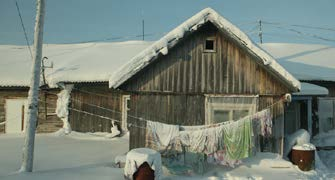
\includegraphics[width=\textwidth]{assets/figures/image}
  \caption{Рисунок}
  \label{fig:fig02}
\end{figure}

\begin{figure}
  \centering
  \includegraphics[height=0.85\textheight]{inc/img/leonardo}
  \caption{Предполагаемый автопортрет Леонардо да Винчи}
  \label{fig:leonardo}
\end{figure}

В \cite{wiki:latex} указано, что... \cite{Pup09}

Кстати, про картинки. Во-первых, для фигур следует использовать \texttt{[ht]}. Если и после этого картинки вставляются <<не по ГОСТ>>, т.е. слишком далеко от места ссылки, "--- значит у вас в РПЗ \textbf{слишком мало текста}! Хотя и ужасный параметр \texttt{!ht} у окружения \texttt{figure} тоже никто не отменял, только при его использовании документ получается страшный, как в ворде, поэтому просьба так не делать по возможности.

\section{Существующие подходы к созданию всячины}

Известны следующие подходы...

\begin{enumerate}
\item Перечисление с номерами.
\item Номера первого уровня. Да, ГОСТ требует именно так "--- сначала буквы, на втором уровне "--- цифры.
Чуть ниже будет вариант <<нормальной>> нумерации и советы по её изменению.
Да, мне так нравится: на первом уровне выравнивание элементов как у обычных абзацев. Проверим теперь вложенные списки.
\begin{enumerate}
\item Номера второго уровня.
\item Номера второго уровня. Проверяем на длииииной-предлиииииииииинной строке, что получается.... Сойдёт.
\end{enumerate}
\item По мнению Лукьяненко, человеческий мозг старается подвести любую проблему к выбору
  из трех вариантов.
\item Четвёртый (и последний) элемент списка.
\end{enumerate}

Теперь мы покажем, как изменить нумерацию на «нормальную», если вам этого захочется. Пара команд в начале документа поможет нам.

\renewcommand{\labelenumi}{\arabic{enumi})}
\renewcommand{\labelenumii}{\asbuk{enumii})}

\begin{enumerate}
\item Изменим нумерацию на более привычную...
\item ... нарушим этим гост.
\begin{enumerate}
\item Но, пожалуй, так лучше.
\end{enumerate}
\end{enumerate}

В заключение покажем произвольные маркеры в списках. Для них нужен пакет \textbf{enumerate}.
\begin{enumerate}[1.]
\item Маркер с арабской цифрой и с точкой.
\item Маркер с арабской цифрой и с точкой.
\begin{enumerate}[I.]
\item Римская цифра с точкой.
\item Римская цифра с точкой.
\end{enumerate}
\end{enumerate}

В отчётах могут быть и таблицы "--- см. табл.~\ref{tab:tabular} и~\ref{tab:longtable}.
Небольшая таблица делается при помощи \Code{tabular} внутри \Code{table} (последний
полностью аналогичен \Code{figure}, но добавляет другую подпись).

\begin{table}[ht]
  \caption{Пример короткой таблицы с коротким названием}
  \begin{tabular}{|r|c|c|c|l|}
  \hline
  Тело      & $F$ & $V$  & $E$ & $F+V-E-2$ \\
  \hline
  Тетраэдр  & 4   & 4    & 6   & 0         \\
  Куб       & 6   & 8    & 12  & 0         \\
  Октаэдр   & 8   & 6    & 12  & 0         \\
  Додекаэдр & 20  & 12   & 30  & 0         \\
  Икосаэдр  & 12  & 20   & 30  & 0         \\
  \hline
  Эйлер     & 666 & 9000 & 42  & $+\infty$ \\
  \hline
  \end{tabular}
  \label{tab:tabular}
\end{table}

Для больших таблиц следует использовать пакет \Code{longtable}, позволяющий создавать
таблицы на несколько страниц по ГОСТ.

Для того, чтобы длинный текст разбивался на много строк в пределах одной ячейки, надо в
качестве ее формата задавать \texttt{p} и указывать явно ширину: в мм/дюймах
(\texttt{110mm}), относительно ширины страницы (\texttt{0.22\textbackslash textwidth})
и~т.п.

Можно также использовать уменьшенный шрифт "--- но, пожалуйста, тогда уж во \textbf{всей}
таблице сразу.

\begin{center}
  \begin{longtable}{|p{0.40\textwidth}|c|p{0.30\textwidth}|}
    \caption{Пример длинной таблицы с длинным названием на много длинных-длинных строк}
    \label{tab:longtable}
    \\ \hline
    Вид шума & Громкость, дБ & Комментарий \\
    \hline \endfirsthead
    \subcaption{Продолжение таблицы~\ref{tab:longtable}}
    \\ \hline \endhead
    \hline \subcaption{Продолжение на след. стр.}
    \endfoot
    \hline \endlastfoot
    Порог слышимости             & 0     &                                                \\
    \hline
    Шепот в тихой библиотеке     & 30    &                                                \\
    Обычный разговор             & 60-70 &                                                \\
    Звонок телефона              & 80    & \small{Конечно, это было до эпохи мобильников} \\
    Уличный шум                  & 85    & \small{(внутри машины)}                        \\
    Гудок поезда                 & 90    &                                                \\
    Шум электрички               & 95    &                                                \\
    \hline
    Порог здоровой нормы         & 90-95 & \small{Длительное пребывание на более
    громком шуме может привести к ухудшению слуха}                                        \\
    \hline
    Мотоцикл                     & 100   &                                                \\
    Power Mower                  & 107   & \small{(модель бензокосилки)}                  \\
    Бензопила                    & 110   & \small{(Doom в целом вреден для здоровья)}     \\
    Рок-концерт                  & 115   &                                                \\
    \hline
    Порог боли                   & 125   & \small{feel the pain}                          \\
    \hline
    Клепальный молоток           & 125   & \small{(автор сам не знает, что это)}          \\
    \hline
    Порог опасности              & 140   & \small{Даже кратковременное пребывание на
    шуме большего уровня может привести к необратимым последствиям}                       \\
    \hline
    Реактивный двигатель         & 140   &                                                \\
                                 & 180   & \small{Необратимое полное повреждение
                                 слуховых органов}                                        \\
    Самый громкий возможный звук & 194   & \small{Интересно, почему?..}                   \\
  \end{longtable}
\end{center}

%%% Local Variables:
%%% mode: latex
%%% TeX-master: "rpz"
%%% End:

% \chapter{Конструкторский раздел}
\label{cha:design}

В данном разделе проектируется новая всячина.

\section{Архитектура всячины}

\subsection{Протестируем подпункт}
\subsubsection{А теперь подподпункт}


\paragraph{Проверка} параграфа. Вроде работает.
\paragraph{Вторая проверка} параграфа. Опять работает.

Вот.

\begin{itemize}
\item Это список с <<палочками>>.
\item Хотя он и по ГОСТ, но\dots
\end{itemize}

\begin{enumerate}
\item  Для списка, начинающегося с заглавной буквы, лучше список с цифрами.
\end{enumerate}

Формула \eqref{F:F1} совершено бессмысленна.

%Кстати, при каких-то условиях <<удавалось>> получить двойный скобки вокруг номеров формул. Вопрос исследуется.

\begin{equation}
a= cb
\label{F:F1}
\end{equation}

А формула~\eqref{eq:fourierrow} имеет некоторый смысл.
Кроме этого она пытается иллюстрировать применение окружения \Code{eqndesc} которое размещает формулу совместно с её описанием.
Однако обратите внимание на нумерацию формул~\eqref{eq:fourierrow} и \eqref{F:F2}, попробуйте добавить \Code{[H]} к такой формуле.

\begin{eqndesc}
    \begin{equation}\label{eq:fourierrow}
        f(x) = \frac{a_0}{2} + \sum\limits_{k=1}^{+\infty} A_k\cos\left(k\frac{2\pi}{\tau}x+\theta_k\right)
    \end{equation}

    где $A_k$ "--- амплитуда  k-го гармонического колебания,\\
    $A_k$ "--- амплитуда $k$-го гармонического колебания,\\
    $ k\frac{2\pi}{\tau} = k\omega$ "--- круговая частота гармонического колебания,\\
    $\theta_k$ "--- начальная фаза $k$-го колебания.
\end{eqndesc}


Окружение \texttt{cases} опять работает (см. \eqref{F:F2}), спасибо И. Короткову за исправления..


\begin{equation}
a= \begin{cases}
 3x + 5y + z, \mbox{если хорошо} \\
 7x - 2y + 4z, \mbox{если плохо}\\
 -6x + 3y + 2z, \mbox{если совсем плохо}
\end{cases}
\label{F:F2}
\end{equation}

\section{Подсистема всякой ерунды}

Культурная вставка dot-файлов через утилиту dot2tex (рис.~\ref{fig:fig02}).

\begin{figure}
  \centering
% [width=0.5\textwidth] --- регулировка ширины картинки
  \includegraphics[width=.5\textwidth]{inc/dot/cow2}
  \caption{Рисунок}
  \label{fig:fig02}
\end{figure}


\subsection{Блок-схема всякой ерунды}

\subsubsection*{Кстати о заголовках}

У нас есть и \Code{subsubsection}. Только лучше её не нумеровать.

%%% Local Variables:
%%% mode: latex
%%% TeX-master: "rpz"
%%% End:

% \chapter{Технологический раздел}
\label{cha:impl}

В данном разделе описано изготовление и требование всячины. Кстати,
в Latex нужно эскейпить подчёркивание (писать <<\verb|some\_function|>> для \Code{some\_function}).

\ifPDFTeX
Для вставки кода есть пакет \Code{listings}. К сожалению, пакет \Code{listings} всё ещё
работает криво при появлении в листинге русских букв и кодировке исходников utf-8.
В данном примере он (увы) на лету конвертируется в koi-8 в ходе сборки pdf.

Есть альтернатива \Code{listingsutf8}, однако она работает лишь с
\Code{\textbackslash{}lstinputlisting}, но не с окружением \Code{\textbackslash{}lstlisting}

Вот так можно вставлять псевдокод (питоноподобный язык определен в \Code{listings.inc.tex}):

\begin{lstlisting}[style=pseudocode,caption={Алгоритм оценки дипломных работ}]
def EvaluateDiplomas():
    for each student in Masters:
        student.Mark := 5
    for each student in Engineers:
        if Good(student):
            student.Mark := 5
        else:
            student.Mark := 4
\end{lstlisting}

Еще в шаблоне определен псевдоязык для BNF:

\begin{lstlisting}[style=grammar,basicstyle=\small,caption={Грамматика}]
  ifstmt -> "if" "(" expression ")" stmt |
            "if" "(" expression ")" stmt1 "else" stmt2
  number -> digit digit*
\end{lstlisting}

В листинге~\ref{lst:sample01} работают русские буквы. Сильная магия. Однако, работает
только во включаемых файлах, прямо в \TeX{} нельзя.

% Обратите внимание, что включается не ../src/..., а inc/src/...
% В Makefile есть соответствующее правило для inc/src/*,
% которое копирует исходные файлы из ../src и конвертирует из UTF-8 в KOI8-R.
% Кстати, поэтому использовать можно только русские буквы и ASCII,
% весь остальной UTF-8 вроде CJK и египетских иероглифов -- нельзя.

\lstinputlisting[language=C,caption=Пример (\Code{test.c}),label=lst:sample01]{inc/src/test.c}

\else

Для вставки кода есть пакет \texttt{minted}. Он хорош всем кроме: необходимости Python (есть во всех нормальных (нет, Windows, я не про тебя) ОС) и Pygments и того, что нормально работает лишь в \XeLaTeX.

\ifdefined\NoMinted
Но к сожалению, у вас, по-видимому, не установлен Python или pygmentize.
\else
Можно пользоваться расширенным BFN:

\begin{listing}[H]
\begin{ebnfcode}
 letter = "A" | "B" | "C" | "D" | "E" | "F" | "G"
       | "H" | "I" | "J" | "K" | "L" | "M" | "N"
       | "O" | "P" | "Q" | "R" | "S" | "T" | "U"
       | "V" | "W" | "X" | "Y" | "Z" ;
digit = "0" | "1" | "2" | "3" | "4" | "5" | "6" | "7" | "8" | "9" ;
symbol = "[" | "]" | "{" | "}" | "(" | ")" | "<" | ">"
       | "'" | '"' | "=" | "|" | "." | "," | ";" ;
character = letter | digit | symbol | "_" ;
 
identifier = letter , { letter | digit | "_" } ;
terminal = "'" , character , { character } , "'" 
         | '"' , character , { character } , '"' ;
 
lhs = identifier ;
rhs = identifier
     | terminal
     | "[" , rhs , "]"
     | "{" , rhs , "}"
     | "(" , rhs , ")"
     | rhs , "|" , rhs
     | rhs , "," , rhs ;
 
rule = lhs , "=" , rhs , ";" ;
grammar = { rule } ;
\end{ebnfcode}
\caption{EBNF определённый через EBNF}
\label{lst:ebnf}
\end{listing}

А вот в листинге \ref{lst:c} на языке C работают русские комменты. Спасибо Pygments и Minted за это.

\begin{listing}[H]
\cfile{inc/src/test.c}
\caption{Пример — test.c} 
\end{listing}
\label{lst:c}

\fi
\fi
% Для вставки реального кода лучше использовать \texttt{\textbackslash lstinputlisting} (который понимает
% UTF8) и стили \Code{realcode} либо \Code{simplecode} (в зависимости от размера куска).




Можно также использовать окружение \Code{verbatim}, если \Code{listings} чем-то не
устраивает. Только следует помнить, что табы в нём <<съедаются>>. Существует так же команда \Code{\textbackslash{}verbatiminput} для вставки файла.

\begin{verbatim}
a_b = a + b; // русский комментарий
if (a_b > 0)
    a_b = 0;
\end{verbatim}

%%% Local Variables:
%%% mode: latex
%%% TeX-master: "rpz"
%%% End:

% \chapter{Экспериментальный раздел}
\label{cha:research}

В данном разделе проводятся вычислительные эксперименты.
А на рис.~\ref{fig:spire01} показана схема мыслительного процесса автора...

\begin{figure}
  \centering
  \includegraphics[width=\textwidth]{inc/svg/pic01}
  \caption{Как страшно жить}
  \label{fig:spire01}
\end{figure}


%%% Local Variables:
%%% mode: latex
%%% TeX-master: "rpz"
%%% End:

% \chapter{Организационно-экономический раздел}
\label{cha:econom}

\section{Протестируем специальные символы.}

И заодно переключение шрифтов.


{\shorthandoff" \texttt{"-{}-* Прямая речь "-{}-{}- <{}<после ,{},тире`{}` неразрывный пробел>{}>}}

{\cyrillicfonttt{\bfseries\itshape\textbackslash{}cyrillicfonttt}
"--* Прямая речь "--- <<после ,,тире`` неразрывный пробел>>.}

{\cyrillicfontsf{\bfseries\itshape\textbackslash{}cyrillicfontsf}
"--* Прямая речь "--- <<после ,,тире`` неразрывный пробел>>.}

{\cyrillicfont{\bfseries\itshape\textbackslash{}cyrillicfont}
"--* Прямая речь "--- <<после ,,тире`` неразрывный пробел>>.}


\blindtext
%%% Local Variables:
%%% mode: latex
%%% TeX-master: "rpz"
%%% End:

% \chapter{Промышленная экология и безопасность}\label{cha:bzd}

\blindtext

\blindlistlist[3]{enumerate}

%%% Local Variables:
%%% mode: latex
%%% TeX-master: "rpz"
%%% End:


\chapter{Анализ опыта и требований в проектировании энергоэффективных зданий и сооружений в Арктике}
В главе авторы рассматривают опыт Российской Федерации и других стран мира в области проектирования энергоэффективных зданий и сооружений в Арктике и в части требований, предявляемых к таковым.
Задачами анализа является обзор опыта и выявление устойчивых закономерностей в процессах реализации зданий, которые расходуют энергию, реализуя максимальный \gls{factor.usefulEnergy} материалов, изделий, оборудования, механизмов.

При проведении \textbf{оценки}, авторы выделяют следующие оцениваемые аспекты, формирующие \textbf{структуру анализа}:
\begin{itemize}
    \item методы регулирования --- \gls{law.lna}, группа \gls{law.lna}, стандарты, информационные системы,
    практики и способы вовлечения населения и других владельцев застраиваемых территорий (застройщиков) в процесс разработки и проектирования энергоэффективных зданий;
    \item опыт реализации --- материалы, методики и технологии, решаемые с их применением задачи строительства и обеспечения энергоэффективности, тенденции их применения. % TO DO Раскрыть и выявить модель, которую описал И. А. Башмаков. Дополнить при необходимости
\end{itemize}


% Команды для генерации заголовков в разделе
\providecommand{\scAssesmentHeader}[1]
{\textbf{Оценка опыта и требований в проектировании энергоэффективных зданий #1}}
\providecommand{\scAssesmentBuildingClass}{Модельные классы застройки}
\providecommand{\scAssesmentBuildingMetrics}{Модельные метрики потребления энергии}
\providecommand{\scAssesmentExp}{Опыт реализации зданий}
\providecommand{\scAssesmentBuildingLaw}{Методы регулирования}

% Верстка вводных частей
\section{Общемировой опыт и парадигма реализации энергоэффективных зданий}


Сокращение добычи природных энергетических ресурсов и, соответственно увеличение их стоимости, с начала XXI века является вызовом для отрасли жилищного строительства в частности и
для проектирования мер развития территорий в целом. Поскольку этот вызов формирует запрос на оптимизацию энергопотребления при развитии территорий во всем мире,
не ограничиваясь арктическими широтами, авторы в данном вводном разделе рассматривают общемировой опыт реализации энергоэффективных зданий в разрезе формирования
общей парадигмы и принципиального подхода к стандартизации процессов энергоэффективного жилого строительства.

Впервые государственную политику в отношении энерго-ресурсосбережения начали проводить в Соединенных Штатах Америки в начале 90-х годов прошлого столетия.
Затем, ряд документов, так называемых <<конвенций>> --- соглашений, были приняты в странах ЕС.
Это были, в первую очередь, государственные законы, стимулирующие внедрение энергосберегающих технологий \cite{2010buee_Sormunen_Finland,2020buee_Sheyna_HabitatEurotechInsertion}. % Возможно найти первоисточник — сами законы?

В странах Европы, Канаде и Соединенных Штатах Америки энергоэффективное мышление при проектировании и эксплуатации зданий имеет наибольшее развитие:
уделяется внимание энергосберегающим процессам и инструментам их реализации на законодательном уровне, на уровне методологии и стандартизации.
В этих странах строят не просто энергоэффективные здания, а так называемые <<зеленые здания>>, к которым применяются регламентируемые по нормам повышенные требования безопасности,
снижения негативного воздействия на окружающую среду.
<<Зеленые здания>>, согласно требованиям норм, способствуют комфортному проживанию людей и учитывают интересы будущего поколения \cite{2020buee_Muhammad_USWastemanagement}.
Проектирование экологически устойчивых зданий, <<зеленое>> эко-проектирование (Green Architecture) \cite{2008buee_wines_green} и технологические инновации в данной области --- одно из самых популярных и
развиваемых направлений.% Канада --- один из лидеров среди них.% Найти подтверждения — статистику и пр. — что Канада — лидер
Так как практически половина потребления всей получаемой от глобальных энергоресурсов энергии % Уточнить цитату и концепты по указанному источнику
приходится на жилые дома и сооружения, то одним из самых очевидных методов ресурсосбережения становится строительство энергоэффективных и пассивных зданий \cite{1979buee_mazria_passive}.


% Обзор систем стандартизации энергоэффективности — описание текстом, матрица
% ##########################################################################################

% TO DO: таблица стандартов с шапкой:
% Наименование стандарта & Юрисдикция (страны действия) & Способ применения (добровольно/как часть НПА) & Описание метрик (что оценивается) & Описание модели (как оценивается)

% С января 2022-го ратифицированная версия действует и в РФ
Существенным отличием в порядке проектирования энергоэффективных зданий от нашей страны является тот факт, что на территории Канады и США действует
специальная рейтинговая система сертификации: The Leadership in Energy \& Environmental Design (LEED)\footnote{рус. <<Лидерство в Энергетическом и Средовом Проектировании>>} \cite{method_US_LEED} .
Система LEED была разработана в 1998 году United States Green Building Council (USGBC) как стандарт измерения проектов энергоэффективных,
экологически чистых и устойчивых зданий для осуществления перехода строительной индустрии к проектированию, строительству и эксплуатации таких зданий.
Важно отметить, что LEED не заменяет собой требования нормативных документов, установленных в той или иной стране государственными ведомствами,
она только дополняет более совершенными, отвечающими запросам современности, критериями оценки качества.

Новый подход помогает решить такие задачи, как снижение уровня потребления энергетических и материальных ресурсов зданием,
снижение неблагоприятного воздействия на природные эко-системы, обеспечение гарантированного уровня комфорта среды обитания человека,
создание новых энергоэффективных и энергосберегающих продуктов, новых рабочих мест в производственном и эксплуатационном секторах,
формирование общественной потребности в новых знаниях и технологиях в области возобновляемой энергетики, формирование у проектировщиков ответственность за
эффективность решений и будущие функции систем \cite{method_US_LEED}.

Кроме законодательных требований к энергоэффективности зданий, государствами используется метод поощрения и стимулирования энергосбережения:
\begin{itemize}
    \item Германия ежегодно выделяет субсидии для реконструкции зданий с использованием энергоэффективных технологий;
    \item В Канаде строительство таких зданий всячески поддерживается на уровне правительства: для эко- проектирования предусмотрены льготные условия и финансовые стимулы в законодательстве;
    \item В Швейцарии инвесторы могут вкладывать денежные средства в строительство зданий с низким энергопотреблением и получить грант от государства;
    \item Во Франции жильцы домов, сданных до 1977 г., решившие утеплить здание --- могут получить скидку и снижение налоговой ставки до 40\% \cite{2016buee_Sheyna_AltenergyWorldtrands}.
\end{itemize}

% Краткие выводы по моделям ИЛИ перенос в выводы по Главе
% ##########################################################################################

% Перенести в опыт применения одной из стран ИЛИ в \section{Общеприменимые в мире строительные технологии}, если таковой потребуется создать
В европейских странах разрабатываются разного рода здания с повышенной энергоэффективностью и пониженным энергопотреблением направленных к уровню <<Zero Energy Building>> \cite{2017buee_MORCK_240}.
В зарубежном опыте при исследовании зданий на дефекты, ухудшающие тепловую эффективность здания, применяются разного рода тепловизионные устройства в режиме <<time-lapse>>,
при котором заметны все тонкости изменения температурного режима здания после изменения температуры наружной окружающей среды \cite{2015bueemethod_FOX_95,2016bueemethod_FOX_317}.
В работе \cite{2014buee_MEMON_870} описываются способы и методы интеграции энергоемких материалов в строительных конструкциях.


Сам факт использования таких материалов имеет хороший потенциал для зданий при сокращении энергопотребления, но требует некоторых инвестиций во время строительства.
Инвестирование и затраты на повышение тепловой эффективности здания выгодны по экологическим и почти по всем экономическим критериям \cite{2017buee_ADAMCZYK_421}.
В данном случае описываются затраты на потребление 1 кВт*ч в здании, при котором у здания со слабой тепловой защитой повышаются затраты на потребление энергетических ресурсов. 
В Китае нормативом, использующимся для оценки гражданских <<зеленых>> зданий, является <<GB-T 50378-2019 Стандарт оценки зеленых зданий>>,
который является переизданным изданием аналогичного норматива 2014 года с повышением требований.


% Перенести в Таблицу стандартов
Система индексов оценки <<зеленых>> зданий включает пять типов показателей: безопасность и долговечность, здоровье и комфорт, удобство проживания,
уровень ресурсосбережения и комфортность окружающей среды. Каждый показатель имеет обязательные и дополнительные требования для получения баллов \cite{2020buee_Gushin_EnergysaveTrends}.




% Перенос в методы регулирования РФ



\section{Колористика в архитектуре Севера}

Проблема цветовых решений городского пространства исследовалась многими специалистами.
Так, в работах В.Ж. Елизарова, В.А. Глинкина, В.П. Белякова, А.В. Ефимова, Э.П. Путинцева рассматривались отдельные аспекты проблемы колористических решений,включая северные города.
В фундаментальных исследованиях А.В. Ефимова, где он ссылается на исследования Жана-Филиппа Ланкло, выявляются два противоположных подхода к колористическому формированию среды города.
Первый из них, исторический, заключается в интеграции архитектуры в природную стилистику окружения. Он берет свое начало с первых построек человека,
использования натуральных строительных материалов. Поэтому для такого подхода характерна монохромная или сдержанная цветовая гамма.
Второй подход, заключающийся в противопоставлении антропогенной среды природе, также находит отражение в мировой практике.
Для него в большей степени характерна полихромия, смелые цветовые решения и явный контраст с окружающей природой.
В качестве примера приводятся небольшие поселения на северных территориях Норвегии и Канады, где в условиях почти круглогодичного природного «цветового голодания» рождаются
яркие колористические решения в застройке \Code{[52]}.

Стоит отметить факт, основанный на наблюдениях: цвет играет важную роль для защиты от воздействия тепловой энергии солнца.
Так, в Туле в 1954 году был проведен эксперимент, в котором часть покрытия аэродромов была выполнена в белом цвете, часть в черном.
За лето глубина оттаивания грунта под черным покрытием составила 2,25 м, тогда как под белым – 1,65 м.
За счет отражающих свойств белого покрытия можно уменьшать воздействие на многолетнемерзлые грунты \Code{[17, с. 44]}.
Формирование единого похода к колористическому решению крупного города – задача на порядок более сложная, чем отдельного здания или маленького поселка,
так как происходит переход от масштаба одного здания к ансамблевому решению или колористическому объединению квартала, района или целого города.
В 2021 году Информационно-аналитическим центром Государственной комиссии по вопросам развития Арктики был опубликован проект «Дизайн-кода арктических поселений» .
Основная цель этого проекта – создание единых требований к оформлению северного города для формирования его уникального облика.
В нем очень подробно изучаются существующие элементы внешнего оформления на примере трех населенных пунктов: Апатиты, Полярный и Никель.
Далее выявляются удачные и неприемлемые решения по размещению вывесок, баннеров, орнаментов, информационных стендов, памятных табличек, элементов навигации и т.д.,
а также даются рекомендации. Данный подход используется с целью облагораживания среды городов, избавления от «замусоривания» разномастными элементами оформления,
что должно послужить на пользу развития городов. Одновременно с этим рассматриваются колористические решения фасадов,
вопросы использования суперграфики как попытки внести разнообразие в среду города.

На наш взгляд, данная рекомендация в «Дизайн-коде арктических поселений» оказывается спорной.
Она объяснима с точки зрения попытки создания гармоничного цветового решения в городе, однако несколько противоречит выводам,
сделанным многими специалистами на основании фундаментальных исследований за 30–40 лет до этого.
Учитывая то, что в рамках этого исследования нам необходимо сформулировать выводы и рекомендации,
то лучшим выходом будет собрать самое ценное из различных концепций и найти «золотую середину».
Нельзя игнорировать исследования, даже если они проведены более тридцати лет назад: их база не меняется,
глубокое исследование исторических мотивов и опыта предыдущих поколений может быть использовано и сейчас.
Одновременно с этим, современные исследования отличаются большей полнотой и актуальностью собранных данных.
Таким образом можно делать новые заключения, опираясь на все доступные данные и адаптируя их к современным реалиям.
В частности, компромиссом по колористике может быть решение по использованию теплых насыщенных оттенков вместо простых «баночных» цветов при окраске фасадов.
В таком случае даже насыщенные цветовые решения, основанные на контрасте, могут гармонично сочетаться с природным окружением и при этом продолжать выполнять практические функции.

Отдельный момент колористического подхода в попытке формирования уникальной среды – это использование стрит-арта на фасадах зданий.
Данный прием позволяет делать даже здания типовой застройки интересными, нетипичными, а также отражать идентичность места, связанную с национальными или культурными традициями (рис. 4).
Рекомендации, связанные с использованием данного вида оформления, связаны с его визуальным восприятием. Так как размеры таких изображений монументальны,
нужно заранее просчитывать точки и углы возможного обзора для реализации их максимального эффекта.
Также хотелось бы отметить, что в Мурманске можно наблюдать преимущественно геометрические и стилизованные примеры данного вида искусства,
тогда как в Якутске они тяготеют к национальным и природным мотивам, что говорит о различной истории и культурных особенностях этих городов.

\begin{figure}[h]
    \begin{center}
        \hfill
        \begin{minipage}[h]{0.42\linewidth}
            \center{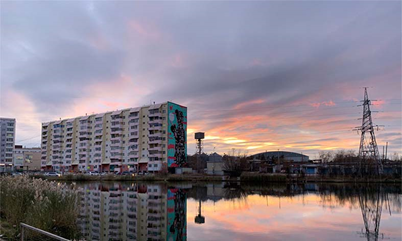
\includegraphics[height=1\linewidth]{assets/figures/st1_colouristic_yakutsk_01.png}} \\ а) 
        \end{minipage}
        \hfill
        \begin{minipage}[h]{0.42\linewidth}
            \center{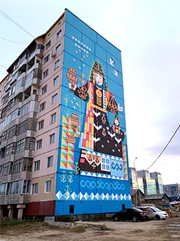
\includegraphics[height=1\linewidth]{assets/figures/st1_colouristic_yakutsk_02.png}} \\б)
        \end{minipage}
        \hfill
    \end{center}
    % \vfill
    \begin{center}
        \hfill
        \begin{minipage}[h]{0.3\linewidth}
        \center{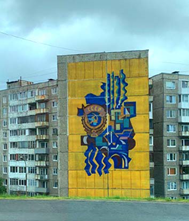
\includegraphics[height=1\linewidth]{assets/figures/st1_colouristic_murom_02.png}} \\ в)
        \end{minipage}
        \hfill
        \begin{minipage}[h]{0.3\linewidth}
        \center{
\includegraphics[height=1\linewidth]{assets/figures/st1_colouristic_murom_03.png}} \\ г)
        \end{minipage}
        \hfill
        \begin{minipage}[h]{0.3\linewidth}
        \center{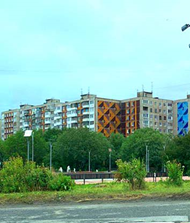
\includegraphics[height=1\linewidth]{assets/figures/st1_colouristic_murom_01.png}} \\ д)
        \end{minipage}
    \end{center}
    \caption{Примеры использования стрит-арта на фасадах зданий (мурал арт) в северных городах.
                Якутск: а) улица Лермонтова, д. 58/2; б) улица Лермонтова, д. 56;
                Мурманск: в) Кольский проспект, д. 142; г) Кольский проспект, д. 138, к. 1; д) улица Зои Космодемьянской, д. 32-36
                }
    \label{fig:st1coloristic_murals}
    \end{figure}

% Верстка раздела с группировкой опыта по странам
\section{\scAssesmentHeader{Российской Федерации}}


% \subsection{\scAssesmentBuildingClass}
% % 
% \subsection{\scAssesmentBuildingMetrics}
% 
% ##########-----Регулирование


\subsection{\scAssesmentBuildingLaw}
% 
В части базы обеспечения стандартизацией процессов регулирования энергетической эффективности законодательством России закреплены национальные стандарты,
описывающие нормативные показатели микроклимата \cite{law_RU_RulesCode_BuildingMicroclimateResedentialPublic} с учётом условий от энергетического воздействия внешней среды \cite{law_RU_RulesCode_BuildingClimatology}
и параметры ограждающих конструкций зданий \cite{law_RU_Rules_Code_ThermalPerformance,law_RU_Rules_Code_BuildingEnclosingConstruction}, оптимизация которых позволяет создавать проектные решения построек,
минимизирующие потери тепловой энергии и мероприятия по снижению затрат на обогрев зданий в целом.
В части базы обеспечения методологии законодательство посредством национальных и межгосударственных стандартов определяет принципиальные подходы (на уровне стратегии)
и методики экономической оценки энергетических систем в зданиях.

Основополагающие концепции для принятия решений, связанных c развитием Арктики, исходят из федерального уровня управления и фиксируются в документах стратегического планирования.
Основания разработки нормативно-правовых актов устанавливают Указы Президента РФ или Приказы ведомств.
На период проведения исследования принят Указ Президента РФ от 5 марта 2020 г. N 164 <<Об Основах государственной политики Российской Федерации в Арктике на период до 2035 года>>.
Согласно Указа, устанавливаются такие методы и механизмы регулирования, как:
\begin{itemize}
    \item издание нормативных правовых актов, регулирующих экономическую и иную деятельность в Арктической зоне Российской Федерации;
    \item разработка и реализация стратегии развития Арктической зоны Российской Федерации и обеспечения национальной безопасности на период до 2035 года, стратегии развития арктического туризма в Российской Федерации;
    \item приведение документов стратегического планирования, разработанных в рамках целеполагания, прогнозирования, планирования и программирования на уровне субъекта Российской Федерации, муниципального образования, а также отраслевых документов стратегического планирования в соответствие с настоящими Основами;
    \item создание единой статистической и информационно-аналитической системы в целях осуществления мониторинга социально-экономического развития Арктической зоны Российской Федерации и управления ее социально-экономическим развитием.
\end{itemize}

На федеральном уровне существуют и дополнительно сформированы формализованные структуры, направленные на работу с арктическими территориям:
\begin{itemize}
    \item Министерство иностранных дел Российской Федерации;
    \item Государственная комиссия по вопросам развития Арктики;
    \item Министерство экономического развития России (Департамент развития межрегионального и приграничного сотрудничества);
    \item Комитет по федеративному устройству, региональной политике, местному самоуправлению и делам Севера Совета Федерации Федерального Собрания Российской Федерации;
    \item Совет по Арктике и Антарктике при Совете Федерации Федерального Собрания Российской Федерации;
    \item Комитет по региональной политике и проблемам Севера и Дальнего Востока Государственной Думы ФС РФ;
\end{itemize}
На уровне субъекта Республики Саха (Якутия) авторами установлены следующие формализованные структуры и институции:
\begin{itemize}
    \item Координационный Арктический совет при Главе Республики Саха (Якутия);
    \item Комитет по вопросам коренных малочисленных народов Севера и делам Арктики Государственного Собрания (Ил Тумэн) Республики Саха (Якутия);
    \item Министерство экономики Республики Саха (Якутия) Государственный комитет Республики Саха (Якутия) по делам Арктики.
\end{itemize}
В соответствии с N 190-ФЗ <<Градостроительный кодекс Российской Федерации>> \cite{law_RU_GradoCodex} правовой основой развития территорий являются
документы территориального планирования (Генеральные планы — в случае развития поселений и населённых пунктов),
определяющие стратегию всей административно-территориальной единицы и функциональное назначение территории как класс функциональной зоны,
и документы градостроительного зонирования (Правила землепользования и застройки), устанавливающие правовые возможности и обязанности застройщиков
в форме градостроительных регламентов на предельно допустимые параметры застройки в соответствии с классом территориальной зоны.

В соответствии с № 261-ФЗ <<Об энергосбережении и о повышении энергетической эффективности и о внесении изменений в отдельные законодательные акты Российской Федерации>>
\cite{law_RU_fz_EnergyEff}, ст. 6, допускается передача полномочий органов государственной власти на региональный уровень. При этом органы власти на уровне субъектов и на уровне местного
самоуправления уполномочены разрабатывать собственные программные документы в области энергоэффективного строительства.

Стандарты по развитию ориентированной на человека среды в насёленных местах, в частности --- в городах, --- на период проведения исследования находятся в разработке.
Публичная версия по завершении разработки будет доступна для ознакомления потенциальным инвесторам и интересантам развития территории \cite{law_RU_govAggregatorArcticStandart}.
Разработку «арктического стандарта» ведет АНО «Информационно-аналитический центр
Государственной комиссии по вопросам развития Арктики» под кураторством Минвостокразвития России и Минстроя России.
Техническая реализация представляет комплекс документов, в котором определены основные принципы и подходы к формированию
комфортной городской среды в соотвествии с потребностями и запросами местных жителей, с учётом климатических условий и особенностей социально-экономического развития городов Арктики.
Эти стандарты также нацелены на комплексный подход со включением опыта строительства и объёмно-планировочных решений из традиционных способов возведения северного дома,
которые с течением времени были апробированы и оптимизированы в части энергоэффективности.

В Российской Федерации с начала 90-х годов прошлого столетия начали серьезно заниматься созданием новой нормативно-правовой базы для повышения энергоэффективности зданий и
в 1995 году впервые было введено нормирование приведенного сопротивления теплопередаче ограждающих конструкций в зависимости от градусо-сутки отопительного периода
и введены изменения в СНиП II-3-79* <<Строительная теплотехника>> \Code{[14]}.

Повышение требований по тепловой защите зданий разделили на два этапа: 1998-2000 гг. и 2001-2005 гг.
Для примера в Таблице \ref{tab:method_gsop_phases} приведены требуемые значения приведенного сопротивления теплопередаче стен, цокольного перекрытия и окон для жилых зданий в условиях г. Якутска.
Также 3 апреля 1996 г. был принят Федеральный закон от N 28-ФЗ "Об энергосбережении" и началась реализация федеральной целевой программы "Энергосбережение России" на 1998 - 2005 годы.
% \begin{equation}
%     R_\text{огрконструкции}^\text{требуемое}\text{, м}{^2} \times \text{°С/Вт}
% \end{equation}

\begin{center}
    \begin{longtable}{|m{0.26\textwidth}|c|c|c|}
        \caption{Требуемые значения приведенного сопротивление теплопередаче конструкций для многоквартирных зданий в г.Якутске по СНиП II-3-79* <<Строительная теплотехника>> с изменениями № 3}
        \label{tab:method_gsop_phases}
        \\ \hline
        \multirow{2}{8cm}{ГСОП, \textdegree C$\times$сут\slash год} & \multicolumn{3}{c|}{$R_\text{огрконструкции}^\text{требуемое}\text{, м}{^2} \times \text{°С/Вт}$}\\
        \cline{2-4}
        & Стены & Покрытия, цокольное перекрытие & Окна \\
        \hline \endfirsthead
        \subcaption{Продолжение таблицы~\ref{tab:method_gsop_phases}}
        \\ \hline \endhead
        \hline \subcaption{Продолжение на след. стр.}
        \endfoot
        \hline \endlastfoot
        1 этап & 2,91 & 4,80 & 0,76             \\
        \hline
        2 этап & 5,09 & 7,48 & 0,76             \\
        \hline
    \end{longtable}
\end{center}

В 2003 г. введен в действие СНиП 23-02-2003 <<Тепловая защита зданий>> \cite{law_RU_Rules_Code_ThermalPerformance} и в нем предусмотрен дополнительно комплексный подход, заключавшийся в ограничении затрат тепла на отопление и вентиляцию. При выполнении указанных условий разрешалось некоторое ослабление требований к отдельным ограждающим элементам. 
В ноябре 2009 года принят Федеральный закон №261 <<Об энергосбережении и о повышении энергетической эффективности…>> \cite{law_RU_fz_EnergyEff}.
В соответствии с этим законом, предусмотрено снижение энергоемкости ВВП России на 40\% к 2020 году и в 2.5. – 3 раза к 2030 году (относительно уровня 2007 года).
В дальнейшем НИИСФ РААСН проведены научно-прикладные работы по гармонизации российских норм по тепловой защите зданий с аналогичными зарубежными нормами развитых стран \Code{[16]}.
В настоящее время оценка новой нормативно-правовой базы показала, что Россия серьезно улучшила позицию в рейтинге среди стран по реализации политики энергоэффективности.
При проектировании тепловой защиты зданий и сооружений \Code{[17]}.

Главным регламентирующим документом выступает СП 50.13330.2012 <<Тепловая защита зданий. Актуализированная редакция СНиП 23-02-2003>> \cite{law_RU_Rules_Code_ThermalPerformance}.
Основные характеристики климата района строительства объектов определяются по СП 131.13330.2020 <<Актуализированная редакция СНиП 23-01-99* Строительная климатология>> \cite{law_RU_RulesCode_BuildingClimatology}.
Основные параметры микроклимата в помещениях зданий регламентируются ГОСТ 30494-2011 <<Здания жилые и общественные. Параметры микроклимата в помещениях>> \cite{law_RU_RulesCode_BuildingMicroclimateResedentialPublic}.

В строительных нормах СП 50.13330.2012 \cite{law_RU_Rules_Code_ThermalPerformance} установлены требования к:
\begin{itemize}
    \item приведенному сопротивлению теплопередаче ограждающих конструкций здания;
    \item удельной теплозащитной характеристике здания;
    \item ограничению минимальной температуры и недопущению конденсации влаги на внутренней поверхности ограждающих конструкций в холодный период года, за исключением светопрозрачных конструкций с вертикальным остеклением (с углом наклона заполнений к горизонту 45° и более);
    \item теплоустойчивости ограждающих конструкций в теплый период года;
    \item воздухопроницаемости ограждающих конструкций;
    \item влажностному состоянию ограждающих конструкций;
    \item теплоусвоению поверхности полов;
    \item расходу тепловой энергии на отопление и вентиляцию зданий.
\end{itemize}


% Рассмотрим некоторые требования из них относительно жилых зданий, строящихся в арктических районах Республики Саха (Якутия). 
% Для проектирования тепловой защиты в соответствие с СП 50.13330.2012 \cite{law_RU_Rules_Code_ThermalPerformance} определяется основной показатель - градусо-сутки отопительного периода (1) в зависимости от места расположения объекта строительства:

\begin{eqndesc}
    \begin{equation}\label{eq:gsop}
        \text{ГСОП}=\ (t_{\text{внутр}}-t_{\text{отпериода}})\times z_{\text{отпериода}}
    \end{equation}

    где $t_{\text{внутр}}$ — расчётная температура внутреннего воздуха, °С,\\
    $t_{\text{отпериода}}$ — средняя температура периода со средней суточной температурой воздуха ниже или равной 8°С (в соответствии с положениями \cite{law_RU_RulesCode_BuildingClimatology}),\\
    $z_{\text{отпериода}}$ — продолжительность (в сутках) периода со средней суточной температурой воздуха ниже или равной 8°С (в соответствии с положениями \cite{law_RU_RulesCode_BuildingClimatology}).
\end{eqndesc}

% ГСОП=(t_в-t_от)×z_от,           (1)
% где t_в – расчетная температура внутреннего воздуха здания, °С;
% t_от, z_от - средняя температура наружного воздуха, °С, и продолжительность, сут/год, отопительного периода.


В настоящее время в России используется следующая классификация энергоэффективности зданий:
рейтинг энергоэффективности здания представлен латинскими буквами A++, A+, A, B+, B, C+, C, C-, D, E, где «A++» представляет наивысший рейтинг,
«C» обозначает обычный уровень, а «E» выражает низший уровень.  Данная классификация регламентируется СП 50.13330.2012 Тепловая защита зданий \cite{law_RU_Rules_Code_ThermalPerformance}
и используется при получении энергетического паспорта здания в Российской Федерации. При этом следует отметить, что  согласно п.10.5 \cite{law_RU_Rules_Code_ThermalPerformance},
присвоение зданию класса "В" и "А" производится только при условии включения в проект следующих обязательных энергосберегающих мероприятий:
\begin{itemize}
    \item устройство индивидуальных тепловых пунктов, снижающих затраты энергии на циркуляцию в системах горячего водоснабжения и оснащенных автоматизированными системами управления и учета потребления энергоресурсов, горячей и холодной воды;
    \item применение энергосберегающих систем освещения общедомовых помещений, оснащенных датчиками движения и освещенности;
    \item применение устройств компенсации реактивной мощности двигателей лифтового хозяйства, насосного и вентиляционного оборудования.
\end{itemize}

Кроме в России приняты ряд стандартов, касающихся обеспечения энергетической эффективности зданий.
ГОСТ Р 54862-2011 \Code{[29]} устанавливает метод определения минимальных требований к функциям систем автоматизации
(далее BACS – building automation and control systems) и технического управления зданий (TBM - technical building management),
которые должны внедряться в зданиях различного назначения; методы оценки влияния указанных функций на потребление энергии зданием,
позволяющие ввести характеристики влияния этих функций в расчеты параметров энергетической эффективности зданий.
В данном стандарте подробно приведены функции управления подсистемами: отоплением, вентиляцией и кондиционированием, освещением, системой автоматизации квартир и всего дома, эксплуатацией и технического обслуживания квартир и всего здания в соответствии классам энегоэффективности зданий.
Кроме того, действуют несколько стандартов, оценивающих экономическую эффективность принимаемых в проекте мероприятий.
ГОСТ 56295-2014 \Code{[30]} и ГОСТ 56502-2015 \Code{[31]} устанавливают требования и правила расчетов экономической эффективности
вариантов энергосберегающих мероприятий в зданиях и выбора наиболее целесообразного варианта реализации таких мероприятий.
Таким образом, повышенные требования по тепловой защите зданий обязывает использование энергоэффективных материалов и технологий при строительстве малоэтажных жилых домов
в арктических районах, и ставит задачу для разработки новых конструктивных решений наружных ограждений.
Однозначно, чтобы достичь требуемые значения сопротивления теплопередаче в наружных ограждающих конструкциях, в первую очередь,
необходимо применять современные теплоизоляционные материалы с низким коэффициентом теплопроводности.
Следует отметить, что в арктических районах республики с учетом высоких расходов на отопление зданий необходимо проектировать жилые дома с высоким классом энергосбережения.


Таким образом, акцент регулирования энергоэффективного строительства в Российской Федерации смещён на регулирование посредством механизмов распределения полномочий в соответствии с принципами
местного самоуправления и разработку методических указаний, которые позволят сформировать базу знаний для внедрения в процесс строительства у разнообразных категорий застройщиков.



% ##########-----Опыт


\subsection{\scAssesmentExp}
% 
В Российской Федерации продолжаются поиский энергетически эффективных подходов в проектировании объёмно-планировочных решений зданий.
Наибольшее влияние на этот процесс оказали разработки В. Щипкова, Б. М. Полуя \cite{1989up_Poluyi_ArchGradoVsurovomKlimate}, К. Г. Туралысова \cite{1996up_Turalysov_BiospherRasseleniye},
труды которых обобщают подходы коренного населения, выработанные при проживании на арктических территориях,
с промышленнными задачами, формирующими требования к расселению, которые были актуальными на период начала промышленного освоения Севера.
В части организации застройки описанные в этих концепциях принципы компактности остаются востребованными и применимыми для формирования энергосберегающей застройки (Рисунок. \ref{fig:st1ch03_ruexp_003}).
\clearpage
\begin{figure}
    \centering
    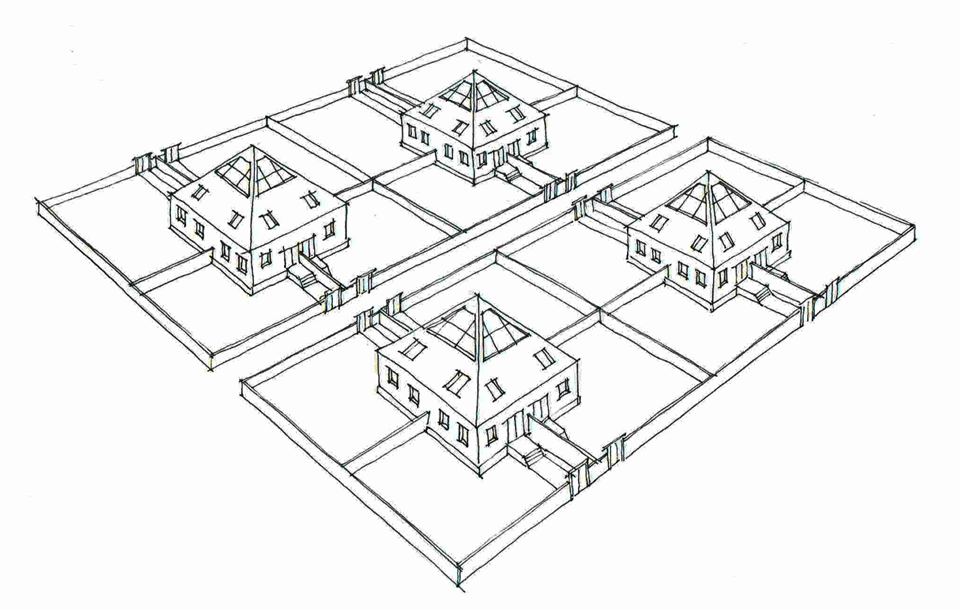
\includegraphics[width=\textwidth]{assets/figures/st1ch03_ruexp_001.png}
    \caption{Концепция компактной энергосберегающей застройки на Севере. Блокированная застройка частными домами}
    \label{fig:st1ch03_ruexp_001}
  \end{figure}

% \clearpage

Принципы энергосберегающей планировки, которые иллюстрируют Рисунки \ref{fig:st1ch03_ruexp_001}, \ref{fig:st1ch03_ruexp_004}, \ref{fig:st1ch03_ruexp_005}, \ref{fig:st1ch03_ruexp_006}, \ref{fig:st1ch03_ruexp_007},
разрабатываемые в рамках концепций застройки, реализуются при вахтовом расслении, на военных базах (Рисунок \ref{fig:st1ch03_ruexp_002}) и научных станциях.


\begin{figure}
    \centering
    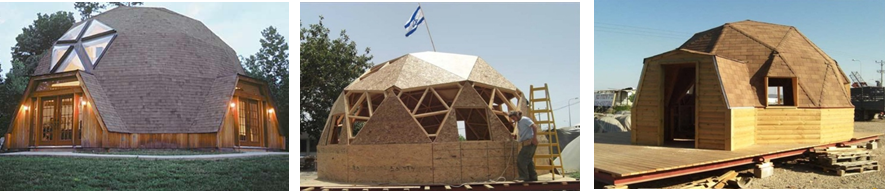
\includegraphics[width=\textwidth]{assets/figures/st1ch03_ruexp_003.png}
    \caption{Уменьшение площади ограждающих конструкций посредством компактной формы постройки в индивидуальном частном домостроении}
    \label{fig:st1ch03_ruexp_003}
  \end{figure}
% \clearpage

\begin{figure}
    \centering
    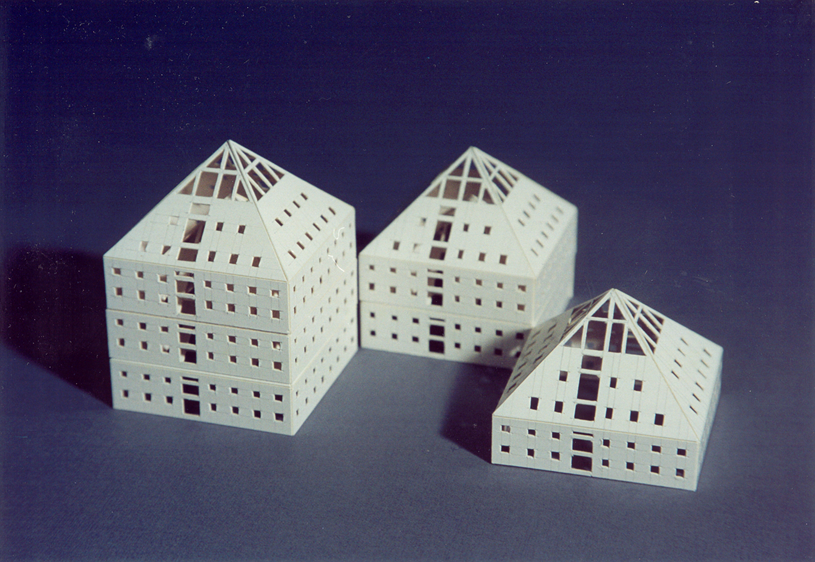
\includegraphics[width=\textwidth]{assets/figures/st1ch03_ruexp_004.png}
    \caption{Концепция компактной энергосберегающей застройки на Севере. Квартирные дома}
    \label{fig:st1ch03_ruexp_004}
  \end{figure}
% \clearpage


\begin{figure}
    \centering
    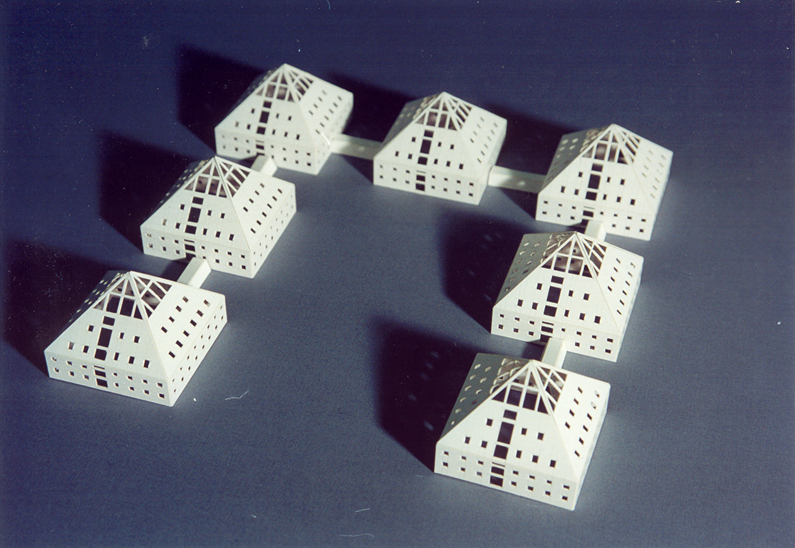
\includegraphics[width=\textwidth]{assets/figures/st1ch03_ruexp_005.png}
    \caption{Концепция компактной энергосберегающей застройки на Севере. Вахтовое расселение}
    \label{fig:st1ch03_ruexp_005}
  \end{figure}


\begin{figure}
    \centering
    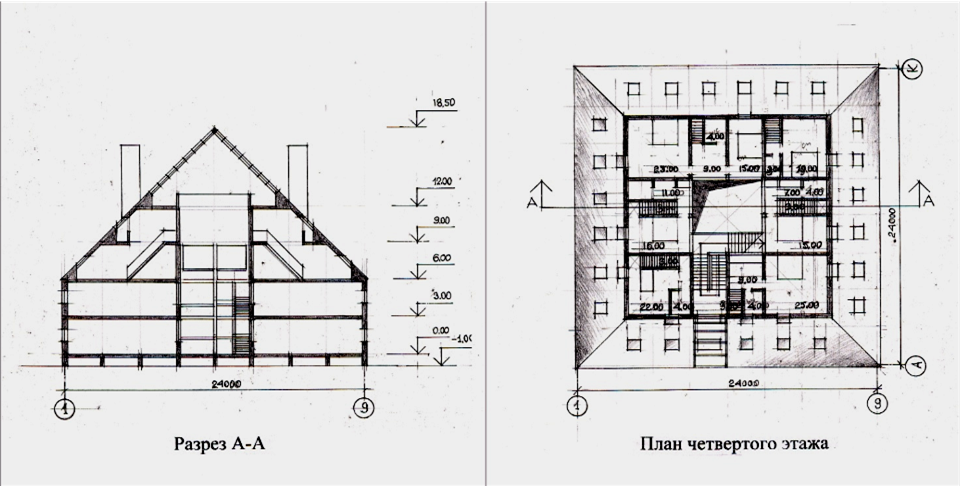
\includegraphics[width=\textwidth]{assets/figures/st1ch03_ruexp_006.png}
    \caption{Концепция компактной энергосберегающей застройки на Севере. Планировочные решения жилого блока}
    \label{fig:st1ch03_ruexp_006}
  \end{figure}


\begin{figure}
    \centering
    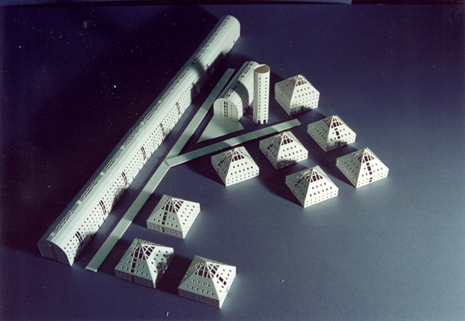
\includegraphics[width=\textwidth]{assets/figures/st1ch03_ruexp_007.png}
    \caption{Концепция компактной энергосберегающей застройки на Севере. Экранирующая противоветровая застройка районов}
    \label{fig:st1ch03_ruexp_007}
  \end{figure}

% \clearpage
\begin{figure}
  \centering
  \includegraphics[width=\textwidth]{assets/figures/st1ch03_ruexp_002.png}
  \caption{Российская военная база <<Арктический трилистник>> на острове Земля Александры (архипелаг Земля Франца Иосифа):
  а - Общий вид военной базы; б, в - Конструктивные особенности военной базы; г - Один из трех эллипсоидных объемов военной базы; д - Интерьер военной базы}
  \label{fig:st1ch03_ruexp_002}
\end{figure}

\begin{figure}
    \centering
    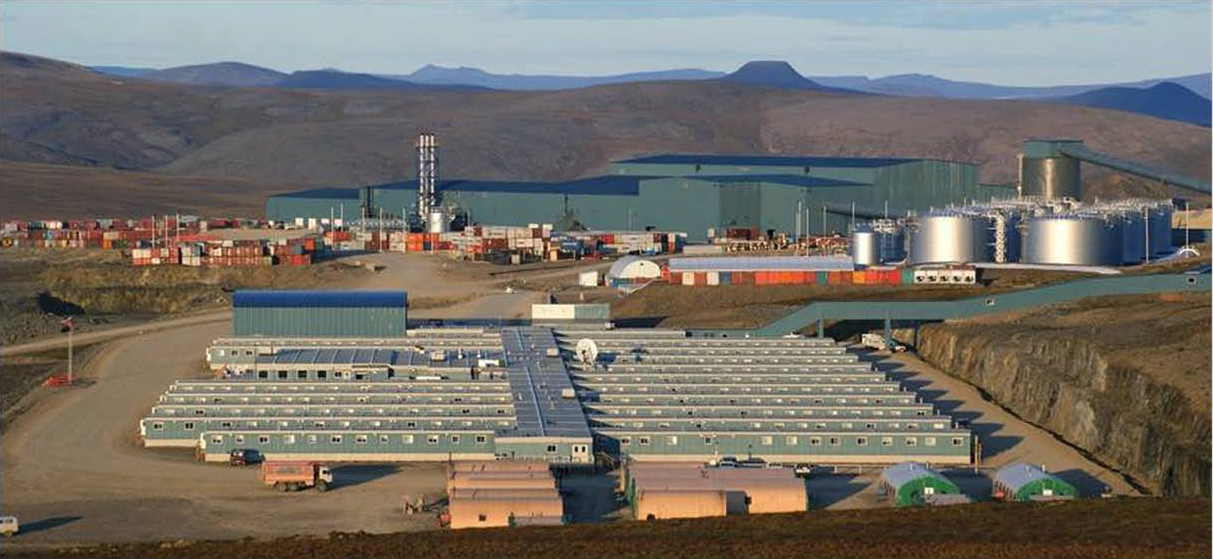
\includegraphics[width=\textwidth]{assets/figures/st1ch03_ruexp_008.png}
    \caption{Вахтовый поселок месторождения Купол, Чукотский автономный округ}
    \label{fig:st1ch03_ruexp_008}
  \end{figure}


\begin{figure}
    \centering
    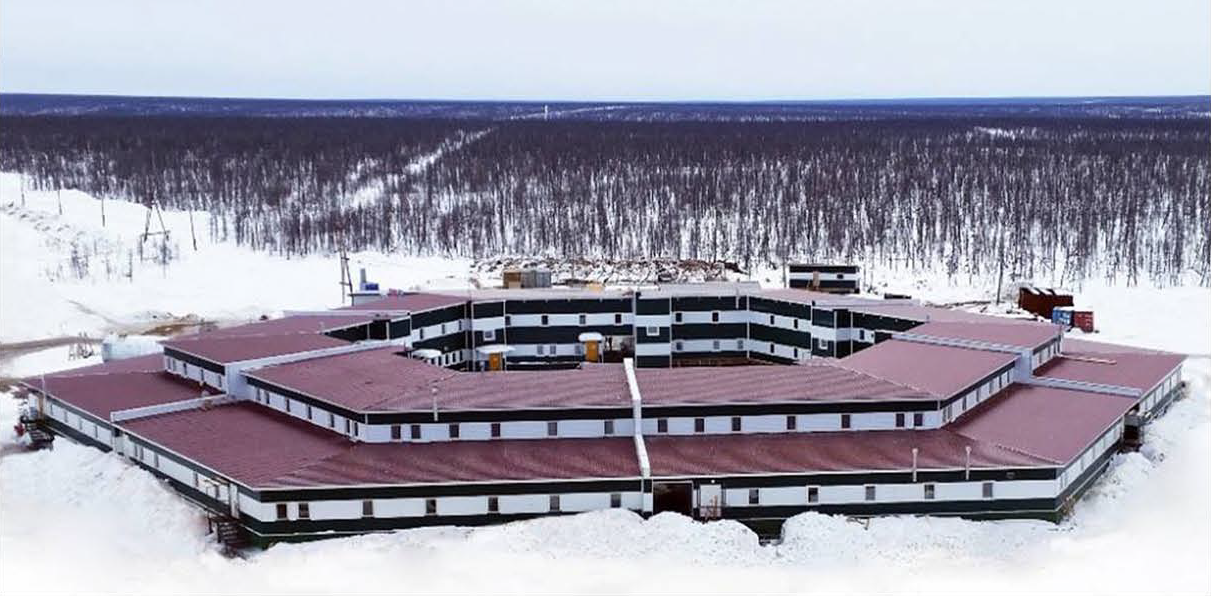
\includegraphics[width=\textwidth]{assets/figures/st1ch03_ruexp_009.png}
    \caption{Вахтовый поселок месторождения Эбелях-Гусиный, Анабарский улус. Республика Саха (Якутия)}
    \label{fig:st1ch03_ruexp_009}
  \end{figure}


\begin{figure}
    \centering
    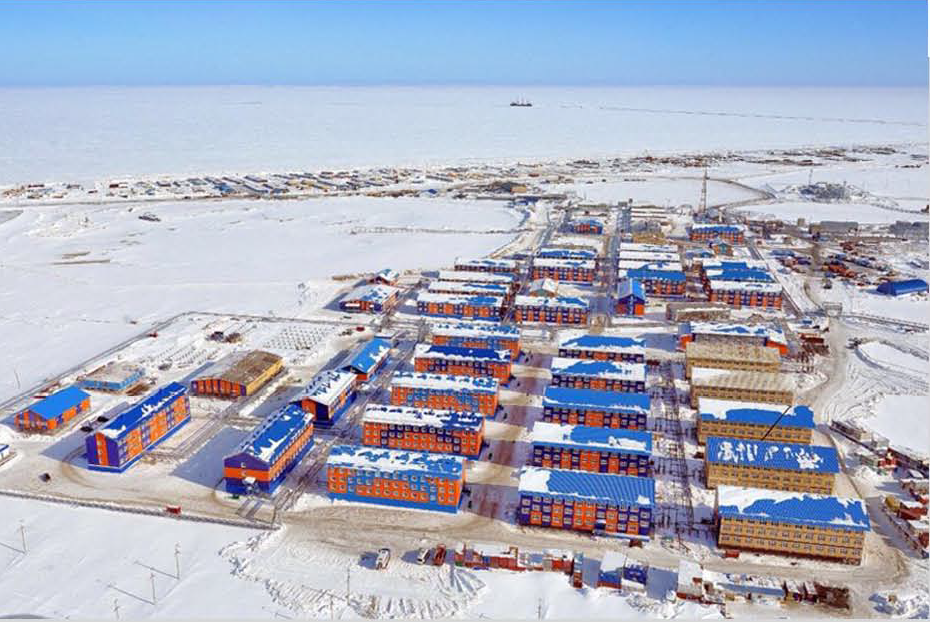
\includegraphics[width=\textwidth]{assets/figures/st1ch03_ruexp_010.png}
    \caption{Вахтовый поселок Сабетта, Ямало-Ненецкий автономный округ}
    \label{fig:st1ch03_ruexp_010}
  \end{figure}


\section{\scAssesmentHeader{Соединённых Штатов Америки}}


\subsection{\scAssesmentBuildingClass}
% 
\subsection{\scAssesmentBuildingMetrics}
% 
\subsection{\scAssesmentBuildingLaw}


\section{\scAssesmentHeader{Канады}}


% \subsection{\scAssesmentBuildingClass}
% % 
% \subsection{\scAssesmentBuildingMetrics}

% ##########-----Регулирование


\subsection{\scAssesmentBuildingLaw}
% 
Нормативная документация для Арктических зон Канады:
\begin{enumerate}[1.]
    \item National Building Code of Canada 2020 --- Национальный строительный кодекс Канады 2020.
    \item Canada building Code in the Context of Climate Change, Adaptation, and Sustainability --- Строительный кодекс Канады в контексте изменения климата, адаптации и устойчивого развития.
\end{enumerate}

% ##########-----Опыт


\subsection{\scAssesmentExp}

В канадской Арктике жильё представлено каркасными домами усадебного типа в стационарных постройках. Кочевники используют палатки и традиционные способы организации быта.
В проектировании и строительстве прослеживаются тенденции на включение бытовых процессов в алгоритм принятия решений при формировании функционально-планировочной организации жилья
и интеграцию опыта коренного населения в технологии строительства в Арктике.
Так, в проекте ARCTIC FOOD NETWORK\footnote{рус. Арктическая продовольственная сеть} \cite{2012_nomads_Canada_AFN}, в программу эксплуатации территории включаются сезонность добычи продовольственных ресурсов, на основе которой выстраивается градостроительное решение на уровне субъекта (уровень схем территориального планирования в терминологии актуального на период исследования российского законодательства \cite{law_RU_GradoCodex}).
Решение направлено на объединение молодого населения на основе традиционного образа жизни с современным переосмыслением, отраженного в рационе коренных жителей Северной Америки инуитов\footnote{отечественному читателю также известных, как <<эскимосы>>}, связанным с промыслом (Рисунок \ref{fig:ch01_s10_sci_AFN01_calendar}).

% \clearpage
\begin{figure}
    \centering
    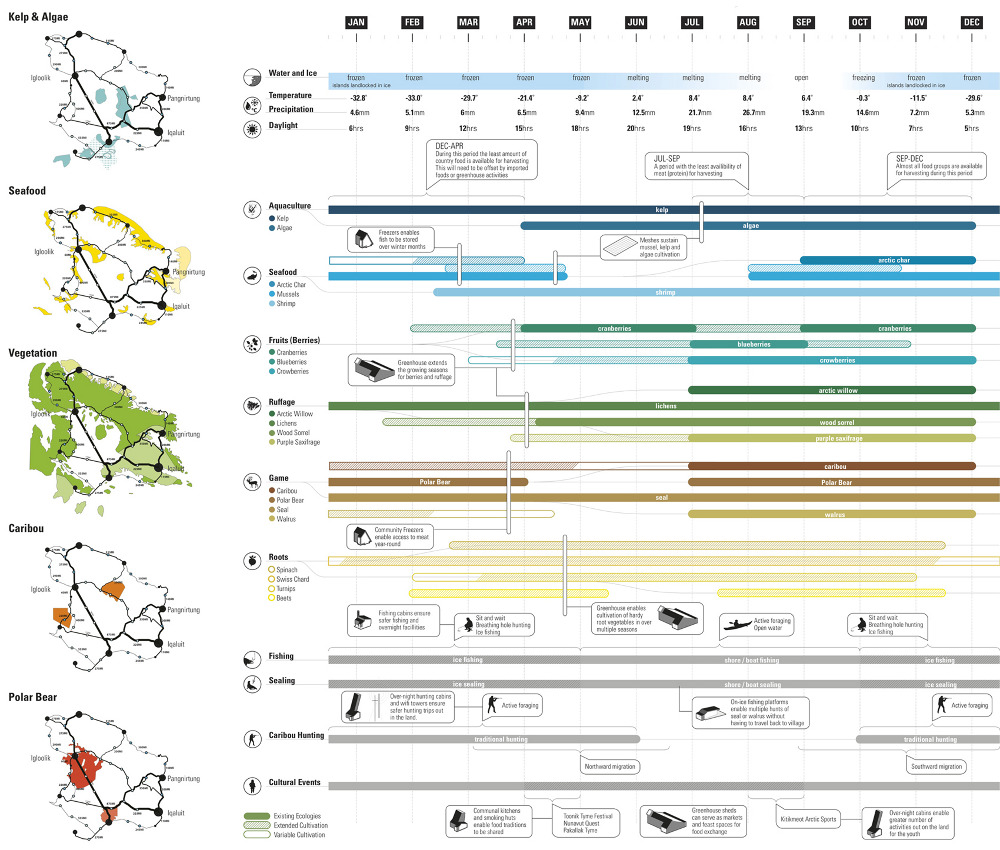
\includegraphics[width=\textwidth]{assets/figures/ch01_s10_sci_AFN01_calendar.png}
    \caption{Календарь проекта, показывающий существующую и проектную сезонность традиционных продуктов питания (графика разработана Lateral Office)}
    \label{fig:ch01_s10_sci_AFN01_calendar}
  \end{figure}

Традиционный рацион инуитов, который сосредоточен на охоте и рыболовстве, постепенно подвергается риску из-за притока пищевых продуктов, произведенных с Юга,
что приводит к увеличению уровня ожирения и диабета. Воздействие такого рациона на здоровье усиливается на Севере из-за высокой стоимости доставки свежих продуктов и более здоровой пищи.
Типичная продовольственная корзина в Нунавуте вдвое дороже аналогичной на Юге Канады, а уровень жизни и зарплаты часто ниже.
Арктическая продовольственная сеть удовлетворяет острую потребность в региональной сети арктических ферм, морозильных камер, и узлах-стоянках.
Сеть окружает большую часть бассейна Фокс в Нунавуте, Канада, ареал разнообразной дикой природы, вдоль побережья Баффиновой Земли и около 30 000 Нунавуммиут.

% \clearpage
\begin{figure}
    \centering
    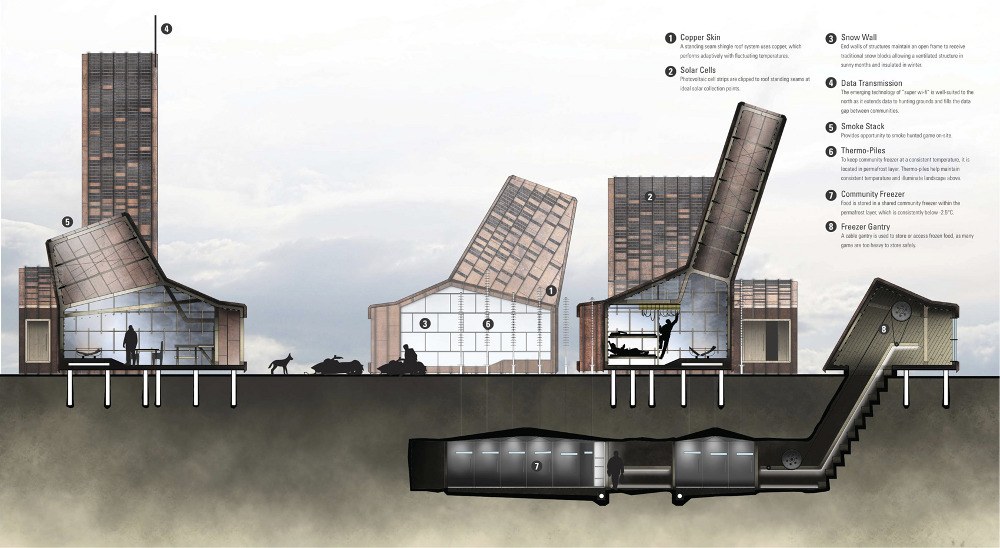
\includegraphics[width=\textwidth]{assets/figures/ch01_s10_sci_AFN01_nodeSection.png}
    \caption{Узел модулей  с кабинами, кухнями и подземными морозильными камерами (графика разработана Lateral Office)}
    \label{fig:ch01_s10_sci_AFN01_nodeSection}
  \end{figure}

Сеть состоит из того, что разработчики из Lateral Office называют навесами, сетками и полюсами, которые относятся к набору уникально интегрированных элементов,
объединяющих архитектуру, ландшафт и технологии. Проект сети - это распределённые узлы регионального сельского хозяйства,
сезонных мест стоянки, центров передачи данных и станций экологического управления. В дополнение к обеспечению безопасной продовольственной и туристической сети,
AFN стремится объединить новые технологии с традиционными практиками для поддержки развивающейся экономики 21-го века.


Таким образом, этот проект наиболее комплексно воплощает все традиционные подходы и адаптации к условиям Арктики,
рассмотренные в предшествующем разделе и реализует эти подходы как на градостроительном уровне, так и в архитектурном проектировании и инженерных решениях.
В этом проекте применяются также узлы примыкания, основанные на традиционных примыканиях в конструктивной схеме инуитского каноэ для промысла,
что является примером тенденции адаптивности инженерных решений к пользователям, создание привычных, дружественных местному коренному населению, методов возведения и обслуживания.


\section{\scAssesmentHeader{Норвегии}}


\subsection{\scAssesmentBuildingClass}
% 
\subsection{\scAssesmentBuildingMetrics}
% 
\subsection{\scAssesmentBuildingLaw}


\section{\scAssesmentHeader{Финляндии}}


% \subsection{\scAssesmentBuildingClass}
% % 
% \subsection{\scAssesmentBuildingMetrics}

% ##########-----Регулирование


\subsection{\scAssesmentBuildingLaw}
% 
Политика на уровне государства направлена на обеспечение мер по преодолению грядущего глобального энергетического кризиса,
государство видит национальную безопасность основой бесперебойных поставок энергии и, в свою очередь, энергию ---
как основу общества и его развития для будущего \cite{law_FIN_govMinEnvSecurity}. Эта позиция находит отражение как основополагающее направление в домостроении.

Большинство финнов живут в частных домах. Одним из основных преимуществ жилья, занимаемого владельцем, по сравнению с арендованным жильем является то,
что часть расходов на жилье, например, взносы по ипотеке, может учитываться как сбережения.

Ministry of the Environment\footnote{рус. Министерство окружающей среды} ведает полномочиями и правовыми актами,
регулирующими взаимодействие человека и жилой среды. Цель министерства окружающей среды заключается в обеспечении адекватного предложения различных видов жилья на рынке жилья,
направлении строительной отрасли и жилищного строительства в направлении, которое является экологически устойчивым, и расширении возможностей жителей влиять на свои жилищные условия.
В министерстве окружающей среды ответственность за жилищное строительство возложена на Департамент антропогенной среды.
Субсидии, субсидии и гарантии, связанные с жильем и строительством, предоставляются Центром финансирования и развития жилищного строительства Финляндии (АРА),
который также руководит и контролирует использование субсидируемого государством строительного фонда АРА.

На уровне субъекта (региональном) действует Regional plan and land use planning, регламентируемый The Land Use and Building Act 132/1999 28 §\footnote{рус. Закон о землепользовании и строительстве},
устанавливющий требования к содержанию регионального плана \cite{law_FIN_RulesCode_LanduseAndBuilding}.
Региональное планирование включает в себя: региональную схему, региональный план, программу регионального развития.
Региональный план представляет собой карту, подготовленную в соответствии с Законом о землепользовании и строительстве, отображающую планы землепользования и структуры общин региона.
В нем описывается строительство и экологическое развитие в ближайшие десятилетия. Региональный план содержит инструкции по муниципальному планированию землепользования и другим официальным мероприятиям, которые влияют на землепользование.
Региональные планы составляются и утверждаются областными советами.
Несколько факторов влияют на муниципальную политику землепользования (планы землепользования и земельная политика).
К ним относятся фактические процессы планирования землепользования и другие виды планирования землепользования, а также промышленная, социальная и жилищная политика.
К числу инструментов планирования землепользования муниципалитетов относятся следующие:
\begin{itemize}
    \item стратегии и программы землепользования в муниципалитете;
    \item местный генеральный план и местный план территории;
    \item земельная политика;
    \item постановление о строительстве.
\end{itemize}
Региональный план определяет, как земля используется в регионе. Местный генеральный план устанавливает цели землепользования в муниципалитете.
В нем излагается общее развитие муниципалитета и использование земельной площади, которую он охватывает, например, расположение жилых районов, мест работы и транспортных маршрутов.
Можно подготовить частичный генеральный план для таких районов, как берега. Такой план может быть более подробным, чем местный генеральный план.
Каждый муниципалитет несет ответственность за подготовку местного генерального плана.
Этот план утверждается муниципальным советом. Если муниципалитеты подготовят общий местный генеральный план, он будет утвержден общим органом муниципалитетов и утвержден министерством окружающей среды.
Закон о землепользовании и строительстве устанавливает требования к содержанию местного генерального плана.
Местный генеральный план используется в качестве основы для подготовки местных подробных планов.


Сбор обратной связи от интересантов территории в ходе разработки документов на всех уровнях принятия решений осуществляется средствами государственных информационных систем
и георафических порталов. В настоящее время в финском государственном управлении проводятся широкомасштабные реформы, направленные на совершенствование управления информацией
и ее использования. Благодаря этим реформам информация, содержащаяся в различных регистрах центральных и местных органов власти, будет соответствовать международным стандартам и
будет более функционально совместимой и пригодной для использования, чем раньше. За информацию о антропогенной среде отвечает главным образом министерство окружающей среды.
Цифровизация административного сектора осуществляется в министерстве в рамках двух широких образований.
Цель состоит в том, чтобы создать основу для общенациональных электронных услуг в сфере недвижимости и строительства, а также для новых возможностей для бизнеса.
Другим аспектом работы в области развития является функциональная совместимость информации о антропогенной среде, поощряемая широкой группой по сотрудничеству.
Вторым объектом является четырехлетний проект Ryhti, который готовит общенациональную информационную систему для антропогенной среды.
Эта работа изложена в Законе о землепользовании и строительстве, который в настоящее время пересматривается.
В его основные задачи входит повышение качества строительства и содействие цифровизации.


Таким образом, регулирование вопросов энергоэффективности зданий Финляндии органично включено в структуру законодательства и реализуется как системный подход,
связанный с территориальным планированием и управлением развитием территориями. Технологии информационного моделирования тесно интегрируются с сообществом и застройщиками,
позволяя реализовать комплексные подходы к оценке и оптимизации параметров энергопотребления зданий при застройке.

% ##########-----Опыт


\subsection{\scAssesmentExp}

Большинство финнов живут в частных домах. Одним из основных преимуществ жилья, занимаемого владельцем, по сравнению с арендованным жильем является то,
что часть расходов на жилье, например, взносы по ипотеке, может учитываться как сбережения. Однако покупка дома обычно влечет за собой получение кредита,
что делает его существенным и долгосрочным. срочное экономическое обязательство, требующее тщательного рассмотрения.
% \clearpage
\begin{figure}
    \centering
    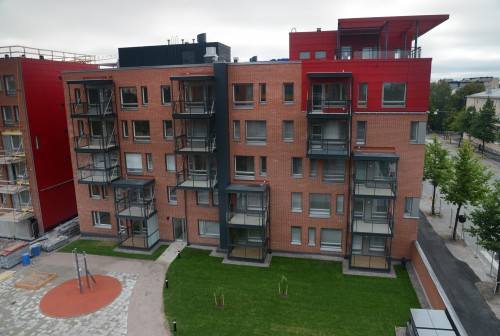
\includegraphics[width=\textwidth]{assets/figures/st1ch03_finexp_001.png}
    \caption{Социальное крупнопанельное жильё в Финляндии (фотоснимок из ресурса https://iti-consulting.ru/dostupnoe-zhile-finskij-opyt-foto/)}
    \label{fig:st1ch03_finexp_001}
  \end{figure}


В крупных населённых пунктах Арктики, таких как Оулу, преобладает микрорайнная застройка блокированными секциями в виде линейных и перемитральных фронтов застройки,
реализуемая с целью компактного распределения инженерных сетей и энергосбережения посредством предотвращения потерь тепла.
Эти объекты возводятся с применением железобетонных каркасов и крупнопанельных модулей (Рисунок \ref{fig:st1ch03_finexp_001}).



\section{\textbf{Выводы}}

В результате оценки опыта и требований в проектировании энергоэффективных зданий и сооружений в Арктике, выделены преобладающие в рассматриваемых странах
технологии строительства, приведённые в Таблице \ref{tab:buildingtech}.

\begin{center}
\begin{longtable}{|m{0.16\textwidth}|m{0.16\textwidth}|m{0.16\textwidth}|l|m{0.16\textwidth}|}
    \caption{Преобладающие в Канаде, США, Российской Федерации, Норвегии и Финляндии технологии строительства жилья}
    \label{tab:buildingtech}
    \\ \hline
    Канада & США & Финляндия & Российская Федерация & Норвегия \\
    \hline \endfirsthead
    \subcaption{Продолжение таблицы~\ref{tab:buildingtech}}
    \\ \hline \endhead
    \hline \subcaption{Продолжение на след. стр.}
    \endfoot
    \hline \endlastfoot
    Каркасно- панельное & Каркасно- панельное & Каркасно- панельное & Каркасно- панельное & Каркасно- панельное  \\
    \hline
    --- & Модульное & Модульное & --- & Модульное  \\
    \hline
    --- & --- & --- & Клеёный брус & Клеёный брус  \\
    \hline
    --- & --- & --- & Оцилиндрованный брус & ---  \\
    \hline
    --- & Крупно- панельное & --- & Крупно- панельное & Крупно- панельное  \\
    \hline
\end{longtable}
\end{center}

Анализом установлено, что требования регулирования в арктических странах совпадают с общемировым вектором трансформации законодательного регулирования в строительстве
и направлены на реализацию комплексного подхода посредством создания социально-информационных площадок на базе государственных информационных систем
и методических указаний для застройщиков.

Информационное моделирование зданий и территорий как средство коммуникации в строительстве и муниципальном хозяйстве наиболее развито в Финляндии: тесно связано с государственными информационными системами мониторинга
и эксплуатации, создаёт наиболее полную и наглядную картину для всех участников строительно-инвестиционных проектов посредством геоинформационных систем и интерактивных визуализаций информационных моделей,
позволяет оперативно получать необходимые знания и государственные услуги в формате <<единого окна>>.

Оценка опыта реализации зданий на арктических территориях рассмотренных стран показывает, что наиболее востребованными являются точечная компактная и блокированная ветрозащитная форма
застройки. В архитектурно-планировочных решениях застройки наибольшую эффективность в сбережении энергии показывают ширококорпусные дома
и точечные здания, в центре которых размещаются инженерные системы, являющиеся основным источником энергии и распространяющие её от центра здания
к наружным ограждающим конструкциям.

% Текст от аспиранток МАРхИ

По материалам изученных исследований специалистов, которые заложили основы теории проектирования северных городов, были выявлены следующие закономерности и составлены рекомендации:
\begin{itemize}
    \item При неровном рельефе и растительности интенсивность снеговетрового потока снижается. Если здание стоит под углом 60-90 градусов к направлению ветра, то является преградой, образует ветровую тень 12-18 Н, где Н – высота дома. Разрыв более 1,5 м и улица вдоль направления ветра: скорость потока увеличивается 1,1-1,3. Въездные площади действую как раструб, который улавливает снегопоток, а прилежащие улицы получают увеличенную скорость ветра. Разрывы до 1 м не влияют, а потому допустимы. Допуск снеговетровых потоков на внутреннюю территорию ухудшает микроклимат. При обтекании снеговетровыми потоками через кровли – уменьшается интенсивность до 0,3. Восстанавливаются через 14-18 Н;
    \item Вывод – нужно создавать преграды-здания с разрывами 5-6Н, что позволит сокращать скорость ветра до 0,4-0,8 Н;
    \item Лесные массивы создают тень на протяжении 200м;
    \item Необходимо создавать снегосборное поле на расстоянии 3-20 км с наветренной стороны (тундра, замерзший водоем далее 1 км и ущелье);
    \item Улицы где будут гулять ветра нужно проектировать шириной в 1,5 раза больше, периметральной застройкой и без перекрестков. Дома ставить в ряд по 3-5. Так упрощается прокладка коммуникаций и удешевляется;
    \item Бытовое ежедневное обслуживаение – в первых этажах и рядом с остановками. Уменьшение радиуса обслуживания (дет сад до 200-250м, школ до 300-400 м, магазинов 300-400, стадионов, зрелищных объектов и тд – 1000-1400. Остановки не менее 9х5 – утепленные, конечные 10х15 с туалетом. Остановки с интервалами 250-300 м;
    \item Благоустройство и организация зон отдыха и спорта: в ветровой тени и инсолируемых местах необходимо предусматривать площадки и озелененные места отдыха.не менее 0,8-1 кв. м на жителя;
    \item Зимние сады необходимо обустраивать, так как северному жителю не хватает зелени. Лучше в верхних этажах со светопрозрачными конструкциями или пристроенных оранжереях;
    \item Если нет многолетней мерзлоты, то можно инженерные коммуникации устраивать под озеленение – оно будет лучше переживать зиму.
\end{itemize}


Для усиления архитектурной выразительности все вышеперечисленное заставляет прибегнуть к использованию ритмометрических приемов, контрасту форм и размеров зданий. Декоративные элементы не помогут добиться эффектной игры светотени (как в южных регионах), поэтому необходимо активно использовать иные декоративные приемы: цветная облицовка стен, муралы. При этом важно учитывать особенности восприятия цвета: из-за уровня освещенности ухудшается тонус центральной нервной системы и, как результат, ухудшается видение предметов. Нужно учитывать, что ахроматические тона естественного ландшафта неблагоприятно влияют на психику, сужая восприятие до примитивных сигналов: белый – есть снег, черный – нет. Цвет выступает хорошим стимулятором, теплые насыщенные цвета положительно влияют на психику.
Одна их главных проблем при проектировании северных городов в советское время – некомплексное развитие. Зачастую первым организовывалось производство, а остальные объекты (жилье и социальные объекты) оставались на втором плане.



\backmatter %% Здесь заканчивается нумерованная часть документа и начинаются ссылки и
            
% \Conclusion % заключение к отчёту

В результате проделанной работы стало ясно, что ничего не ясно...

%%% Local Variables: 
%%% mode: latex
%%% TeX-master: "rpz"
%%% End: 
%% заключение


% % Список литературы при помощи BibTeX
% Юзать так:
%
% pdflatex rpz
% bibtex rpz
% pdflatex rpz

\bibliographystyle{./BibTeX-Styles/ugost2003s}
% Подключить библиографию из каталога ./bibliography/2022/...
\bibliography{
    ./bibliography/2022/common_laws,
    ./bibliography/2022/research_arcticbuildtech_sciAndResearches,
    ./bibliography/2022/research_arcticbuildtech_urbanPlanningTexts
}

%%% Local Variables: 
%%% mode: latex
%%% TeX-master: "rpz"
%%% End: 



\appendix   % Тут идут приложения

% \chapter{Картинки}
\label{cha:appendix1}

\blindtext
\begin{figure}
\centering
\caption{Картинка в приложении. Страшная и ужасная.}
\end{figure}

%%% Local Variables: 
%%% mode: latex
%%% TeX-master: "rpz"
%%% End: 


% \chapter{Еще картинки}
\label{cha:appendix2}
\blindtext

\begin{figure}
\centering
\caption{Еще одна картинка, ничем не лучше предыдущей. Но надо же как-то заполнить место.}
\end{figure}

%%% Local Variables: 
%%% mode: latex
%%% TeX-master: "rpz"
%%% End: 


\end{document}

%%% Local Variables:
%%% mode: latex
%%% TeX-master: t
%%% End:
